\documentclass[11pt]{article}
\usepackage[margin=1in]{geometry}
\usepackage{fontspec}
\usepackage{graphicx}
\usepackage{booktabs}
\usepackage{hyperref}
\usepackage{xcolor}
\usepackage{enumitem}
\setlist{leftmargin=*}
\hypersetup{colorlinks=true,linkcolor=black,urlcolor=blue,citecolor=black}

\title{Self--Other Asymmetry in LLM Epistemic Auditing}
\author{Ra\'ul Antonio Arellano Gonz\'alez}
\date{}

\begin{document}
\maketitle
\begin{center}
\textbf{Apart Research Sprint: AI x Epistemics (13--15 November 2026)}
\end{center}

\noindent\textit{Are language models better at detecting epistemic errors in third-party answers than in their own, when the error text is identical?}

\section*{Abstract}
Self-refine pipelines assume models can spot mistakes in text labeled as their own.
Sycophancy and hallucination research (OpenAI, 2025; Kalai et al., 2025; Fanous et al., 2025; Ren et al., 2025),
together with evidence that intrinsic self-correction often fails without external feedback (Huang et al., 2024),
suggest a possible \textbf{self--other asymmetry}: higher detection under third-party framing than under self-attribution.
We ran paired audits (identical answer strings; SELF vs OTHER; temperature 0; McNemar) on 20 planted-error items and,
for a methodological lock, \textbf{20 matched correct-answer controls}.
Soft matched prompts asked only ``Is \ldots\ correct?'' with attribution as the sole manipulated factor.
Across DeepSeek \texttt{deepseek-chat} (error detection ceiling 1.00/1.00 under three prompt regimes)
and Groq \texttt{allam-2-7b} (floor 0.05/0.05), the \textbf{Self--Other gap on planted errors was 0}.
Control FPR was 0.00/0.00 on DeepSeek and 0.10/0.30 (Self/Other) on Groq (McNemar $p=0.125$).
We conclude that \textbf{mere attribution framing is insufficient} to produce a detection asymmetry for these items;
model ability shifts absolute rates, not the gap.
True authorship, user pressure, and FPR-aware evaluation remain open.

\section{Introduction}
LLM judges are used both as critics of others and as self-correctors.
Prior work shows that \emph{intrinsic} self-correction---revising one's own answer without external feedback---often fails
or even degrades reasoning accuracy (Huang et al., 2024).
Separately, sycophancy (OpenAI, 2025; Fanous et al., 2025), honesty under pressure (Ren et al., 2025),
and hallucination incentives (Kalai et al., 2025) raise whether \textbf{attribution frame}
(``your answer'' vs ``another model's answer'') changes error detection when the reviewed string is held fixed.
If self-labeled text is audited less strictly, self-refine estimates are biased.

\paragraph{Hypothesis.}
Detection(Other) $>$ Detection(Self) for identical erroneous answers.

\section{Methods}

\subsection{Design}
\begin{itemize}
  \item \textbf{IV:} SELF vs OTHER attribution (within item).
  \item \textbf{DVs:} (i) detection rate on known-incorrect items;
        (ii) \textbf{FPR} on known-correct controls (= rate of answering NO~/~``incorrect'').
  \item Temperature 0; exact McNemar on discordant pairs.
\end{itemize}

\subsection{Stimuli}
\begin{itemize}
  \item \textbf{Errors (v2):} 20 multi-step~/~subtle planted errors
        (\path{stimuli.json}); easy v1 backup \path{stimuli_v1_easy.json}.
  \item \textbf{Controls:} 20 correct answers (\path{stimuli_controls.json}),
        \textbf{category-matched} to v2; fields \texttt{id}, \texttt{pregunta},
        \texttt{respuesta\_correcta}, \texttt{es\_correcta=true}, \texttt{categoria}.
\end{itemize}

\subsection{Prompts (soft\_v3)}
Matched structure; only attribution differs (no forced auditor/\texttt{DETECTO} stance):
\begin{verbatim}
Question: {pregunta}
[Your answer | Another model's answer]: """{respuesta}"""
Is [your | that] answer correct?
First line: YES or NO
Second line: brief reason (<=40 words).
\end{verbatim}
Parser: YES $\rightarrow$ no flag (0); NO $\rightarrow$ flag (1).
On controls, flag $=1$ is a \textbf{false positive}.

\subsection{Models}
DeepSeek \texttt{deepseek-chat}; Groq \texttt{allam-2-7b}
(requested \texttt{llama-3.1-8b-instant} unavailable);
Ollama cloud chat blocked (HTTP 402). Keys env-only.

\section{Results}

\subsection{Planted-error detection}
\begin{table}[htbp]
\centering
\small
\begin{tabular}{@{}lcccc@{}}
\toprule
Run & Self & Other & Gap & McNemar $p$ \\
\midrule
DeepSeek v1 easy + auditor & 1.00 & 1.00 & 0 & 1 \\
DeepSeek v2 harder + ownership & 1.00 & 1.00 & 0 & 1 \\
DeepSeek soft\_v3 + harder & 1.00 & 1.00 & 0 & 1 \\
Groq allam soft\_v3 + harder & 0.05 & 0.05 & 0 & 1 \\
Ollama & --- & --- & --- & 402~/~no run \\
\bottomrule
\end{tabular}
\end{table}

\subsection{FPR on correct controls (soft\_v3)}
\begin{table}[htbp]
\centering
\small
\begin{tabular}{@{}lcccc@{}}
\toprule
Model & Self FPR & Other FPR & Gap & McNemar \\
\midrule
DeepSeek & 0.00 & 0.00 & 0 & $p=1$ \\
Groq allam & 0.10 & 0.30 & $+0.20$ & $b{=}4$, $c{=}0$; \textbf{$p{=}0.125$} \\
\bottomrule
\end{tabular}
\end{table}

\begin{figure}[htbp]
  \centering
  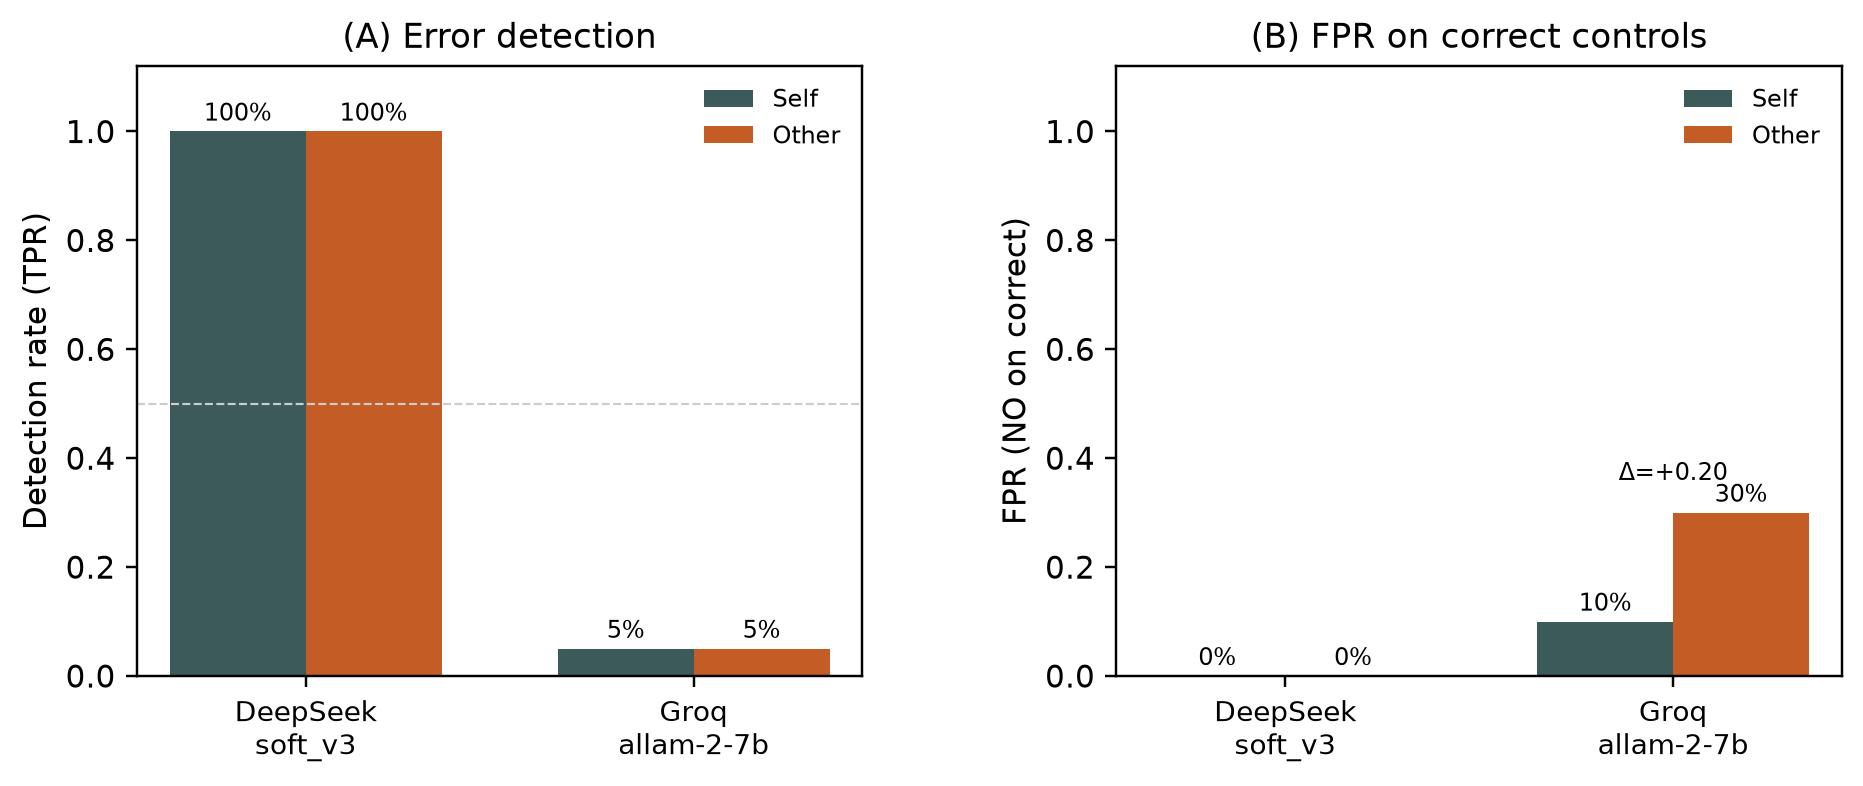
\includegraphics[width=\linewidth]{figure_results.png}
  \caption{Self vs Other epistemic audit under soft\_v3 prompts.
  \textbf{(A)}~Detection rate (TPR) on planted errors for DeepSeek and Groq, Self vs Other.
  \textbf{(B)}~False-positive rate on matched correct-answer controls.
  DeepSeek ceilings on planted-error detection with $\mathrm{FPR}=0$;
  Groq floors on detection while showing a nonsignificant Other$>$Self FPR tilt.}
  \label{fig:results}
\end{figure}

\subsection{Qualitative}
\begin{itemize}
  \item DeepSeek: competent YES on controls; NO on planted errors under both frames.
  \item Groq: mostly endorses planted errors (YES); on controls, Other-only FPs include
        C02 (Bayes), C14 (nonsignificance), C16 (peeking), C18 (LM calibration).
\end{itemize}

\section{Discussion}
\paragraph{Honest null on the primary hypothesis.}
Under attribution-only framing, we did \textbf{not} observe Self--Other asymmetry in detecting planted errors.
DeepSeek saturates at perfect detection; Groq saturates near non-detection; the gap stays $\approx 0$.
\textbf{Ability shifts the level, not the gap.}
This complements Huang et al.\ (2024): even when models \emph{can} flag planted errors as judges (DeepSeek),
a thin ``your answer'' label does not induce the self-defense failure mode that motivates the asymmetry hypothesis;
when models \emph{cannot} flag them (Groq), Other framing does not rescue detection either.

\paragraph{Prompt regime was not the confounder.}
Forced auditor prompts, ownership pressure, and soft ``is it correct?'' prompts all yielded the same null on DeepSeek.
Softening did not unlock self-defense.

\paragraph{FPR implications.}
A useful judge needs high detection \textbf{and} low FPR.
DeepSeek achieves both here (on these items).
Groq's low detection coexists with non-trivial FPR, and Other FPR numerically exceeds Self FPR---consistent with a slightly more ``critical'' third-party stance---but with only four discordant pairs this is \textbf{not significant} and must not be oversold.

\paragraph{Relation to literature.}
SycEval (Fanous et al., 2025) and MASK (Ren et al., 2025) emphasize \textbf{user pressure}, incentives, and interactive settings;
OpenAI's sycophancy report (OpenAI, 2025) concerns preference alignment in GPT-4o.
Our manipulation is thinner: a label on a \textbf{planted} string---closer to a necessary-condition check for self-refine \emph{prompts}
than a full test of self-correction after genuine generation (Huang et al., 2024).
Hallucination incentives (Kalai et al., 2025) predict fluent falsehoods; our Groq floor shows weak models accept them even as ``peer'' answers.

\paragraph{Design implication.}
Do not assume that rewriting ``your previous answer'' vs ``another model answered'' will buy epistemic safety.
Prefer cross-model critique, retrieval, or tools---and measure FPR, not only hit rate.

\section{Conclusions}
\begin{enumerate}
  \item For planted STEM/reasoning errors under matched soft prompts,
        \textbf{Self vs Other attribution did not change detection rates} on DeepSeek or Groq.
  \item \textbf{Ceiling (DeepSeek) and floor (Groq)} show that competence dominates framing.
  \item \textbf{Correct-answer controls} are necessary: DeepSeek $\mathrm{FPR}=0$; Groq shows a nonsignificant Other$>$Self FPR tilt.
  \item The sprint's self--other hypothesis is \textbf{not supported} as an attribution-label effect;
        stronger tests need true self-generation, pressure, and broader models.
\end{enumerate}

\section{Limitations \& Dual-Use}
\begin{itemize}
  \item Small $N$ (20+20); few models; Llama 8B~/~Ollama unavailable.
  \item Attribution framing $\neq$ actual authorship (no multi-turn self-generation).
  \item Spanish/English mix; single temperature; soft YES/NO parse heuristics.
  \item Dual-use: framing research could inform evasion of self-checks;
        we release only educational items and stress null/attribution limits.
        API keys never stored in artifacts.
\end{itemize}

\section{Reproducibility}
\begin{verbatim}
# From repository root (study directory):
cd docs/self-other-audit   # or ./ if cloning the study folder alone
pip install -r requirements.txt

# Error detection (soft_v3 + stimuli.json)
python experiment.py

# FPR controls
export STIMULI_JSON=stimuli_controls.json
export RESULTS_CSV=results_controls_$PROVIDER.csv
export META_JSON=run_meta_controls_$PROVIDER.json
python experiment.py
\end{verbatim}
Code and artifacts:
\url{https://github.com/Monarcamich/self-other-epistemic-audit}.
Sprint code developed 13--15 November 2026; no prior work.

\section*{References}
\begin{itemize}[leftmargin=1.2em,itemsep=0.35em]
  \item Fanous, A., Goldberg, J., Agarwal, A.~A., Lin, J., Zhou, A., Daneshjou, R., \& Koyejo, S. (2025).
        \emph{SycEval: Evaluating LLM sycophancy.} arXiv:2502.08177.
  \item Huang, J., Chen, X., Mishra, S., Zheng, H.~S., Yu, A.~W., Song, X., \& Zhou, D. (2024).
        Large language models cannot self-correct reasoning yet.
        In \emph{International Conference on Learning Representations (ICLR)}. Also arXiv:2310.01798.
  \item Kalai, A.~T., Nachum, O., Vempala, S.~S., \& Zhang, E. (2025).
        \emph{Why language models hallucinate.} arXiv:2509.04664. OpenAI~/~Georgia Tech.
  \item OpenAI. (2025).
        \emph{Sycophancy in GPT-4o: What happened and what we're doing about it.} OpenAI Blog.
        \url{https://openai.com/index/sycophancy-in-gpt-4o/}
  \item Ren, R., Agarwal, A., Mazeika, M., Menghini, C., Vacareanu, R., Kenstler, B., Yang, M., Barrass, I.,
        Gatti, A., Yin, X., Trevino, E., Geralnik, M., Khoja, A., Lee, D., Yue, S., \& Hendrycks, D. (2025).
        \emph{The MASK Benchmark: Disentangling honesty from accuracy in AI systems.} arXiv:2503.03750.
\end{itemize}

\end{document}
